\documentclass[10pt]{article}

\usepackage{lipsum}
\usepackage{url}
\usepackage{float}
\usepackage{amsmath}
\usepackage{enumitem}
\usepackage{graphicx}
\usepackage{caption}
\usepackage{subcaption}
\usepackage{rotating}
\usepackage{geometry}
\usepackage{listings}
\usepackage{hyperref}
\usepackage[T1]{fontenc}
\usepackage{siunitx}
\usepackage[numbered]{matlab-prettifier}

\newcommand{\documentTitle}{Lab 4 - Signal Processing II: Active Circuits}
\newcommand{\documentAuthor}{Andrew Pham, Aneel Damaraju}
\newcommand{\courseTitle}{ELEC 240}
\newcommand{\testDate}{September 26, 2018}
\newcommand{\reportDate}{October 2, 2018}

\geometry{margin=1in}
\lstset{
    tabsize=4,
    basicstyle={\ttfamily},
    captionpos=b,
    belowskip=1em,
    aboveskip=1em,
    numbers=left,
	escapechar=\@,
}

\title{
    \textbf{\courseTitle} \\
    \textbf{\documentTitle} \\
    \bigskip
    \textbf{\large{Test performed: \testDate}} \\
    \textbf{\large{Report submitted: \reportDate}} \\
    \bigskip
    \bigskip
}
\author{\documentAuthor}
\date{}

\begin{document}

\maketitle

\newpage

\section{Objective}

In this lab, we worked on understanding the workings of both breadboards and Op-Amps. We learned how to wire and set up a breadboard for future use, a well as initialize an Op-Amp in your circuit. Experimental values were compared to calculated ones through the use of the oscilloscope. We learned how to create an inverting amplifier and how the values are gated by the DC offset as well as the power supply. Fiially,zen preparation for the lab next week, we assembled a circuit containing two microphones and a speaker in order to transmit and amplify external signals coming in the form of audio waves.

\section{Materials}
\begin{itemize}
	\item Breadboard
	\item 741 Op Amp
	\item NI Virtual Bench
	\item \SI{10}{\ohm} Resistor
	\item \SI{100}{\ohm} Resistor
	\item \SI{10}{\kilo\ohm} Resistor (2)
	\item \SI{100}{\kilo\ohm} Resistor
	\item \SI{.1}{\micro\farad} Capacitor
	\item Dynamic Microphone
	\item Telephone handset
\end{itemize}


\section{Test Description}
\subsection{The 741 Op Amp}
After learning about the Op Amp, we compared open and closed loop configurations, and understood the concepts of DC offset amplification and clipping. By creating simple circuits in this format, we familiarized ourselves with the pins on the 741 Op Amp, and creating functional circuits that would not blow out the device.
\subsection{The Inverting Configuration}
In this smaller section of the lab, we focused on the functions of closed loop inverting amplifier configurations of the Op Amp. We learned about topics such as clipping and the slew rate, and how the internal properties of the Op Amp effect the output signal in comparison to the expected output.
\subsection{Transducer Amplifiers}
As the name implies, in this section we used what we knew about Op Amps to create an amplifier that worked on the audio signals created by a dynamic microphone. These signals were first viewed by the Virtual Bench, until the voltage was amplified to an acceptable level. Then, this circuit was attached to the circuit for a phone handset, to show that the Op Amp amplified the audio signal as well. 

\subsection{Pre-Lab Calculations and Schematics}

\begin{centering}
	\begin{figure} [H]
		\centering
		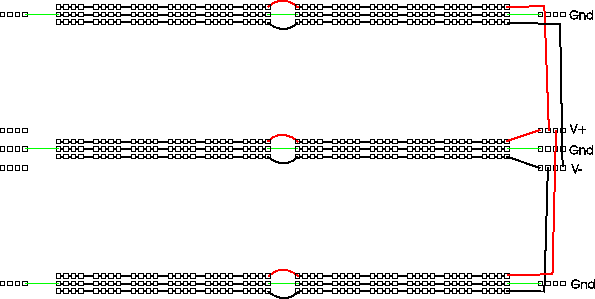
\includegraphics[scale=0.65]{images/Breadboard.png}
		\caption{The wiring needed to properly connect the power across the entire breadboard, as seen, the busses are horizontally, so +15V, GND and -15V power flows horizontally}			
		\label{fig: Breadboard}
	\end{figure}
\end{centering}

Before the lab, there we no calculations to be done, just some setup for the breadboard. To power all of the terminals we needed to set up the power bus, by connecting it to all 3 of the power rails as seen in Fig \ref{fig: Breadboard}. After the power was properly connected, we noted the proper connections for the Interface Board connectors, which would be needed in the lab.

\section{Results and Discussion}

\qquad After setting up the Op-Amp into an open-loop response configuration in Part A for Experiment 4.1, we produced a 2 $V_{pp}$, 20 Hz sine wave. We measured the voltage output from the Op-Amp and observed a max voltage of 14.4 V and a minimum voltage of -13.6 V. We then connected a 100 $\Omega$ resistor between $v_{OUT}$ and ground. This caused the voltage to drop dramatically because the resistor itself has a significant voltage drop. We now observed a max voltage of 3.12 V and a minimum voltage of -1.64 V. After removing the 100 $\Omega$ resistor, we set the function generator to produce a square wave of the same frequency. We observed that $v_{OUT}$ becomes a square wave as well. We also noted some slew-rate limiting, where the slope of $v_{OUT}$ does not change as quickly as $v_{IN}$ when switching between high and low voltages. Furthermore, we noticed that $v_{OUT}$ exhibited 0.79V of DC offset despite the fact that the function generator was set to 0 DC offset. We hypothesized that this DC offset arises from the Op-Amp affecting the input voltage so that it is not perfectly magnified, thus yielding a nonzero DC offset. 

\quad Overall, using an open-loop response configuration is not ideal due to the fact that distortions in the circuit are highly magnified. For example, the small DC offset in the Op-Amp was magnified to nearly a full volt, which caused clipping in the output signal (where the larger amplitude portions of the signal are cut off due to the limitations of the Op-Amp's power supply.)\\\\

\quad We then built an inverting amplifier in Part A of Experiment 4.2 using 10 $k\Omega$ resistors for $R_1$ and the feedback resistor $R_F$. We then set the function generator to produce a 1 $V_{pp}$, 100 Hz sine wave and observed the following output from CH 2 in Fig \ref{fig:invertingamp}. 

\begin{centering}
	\begin{figure} [H]
		\centering
		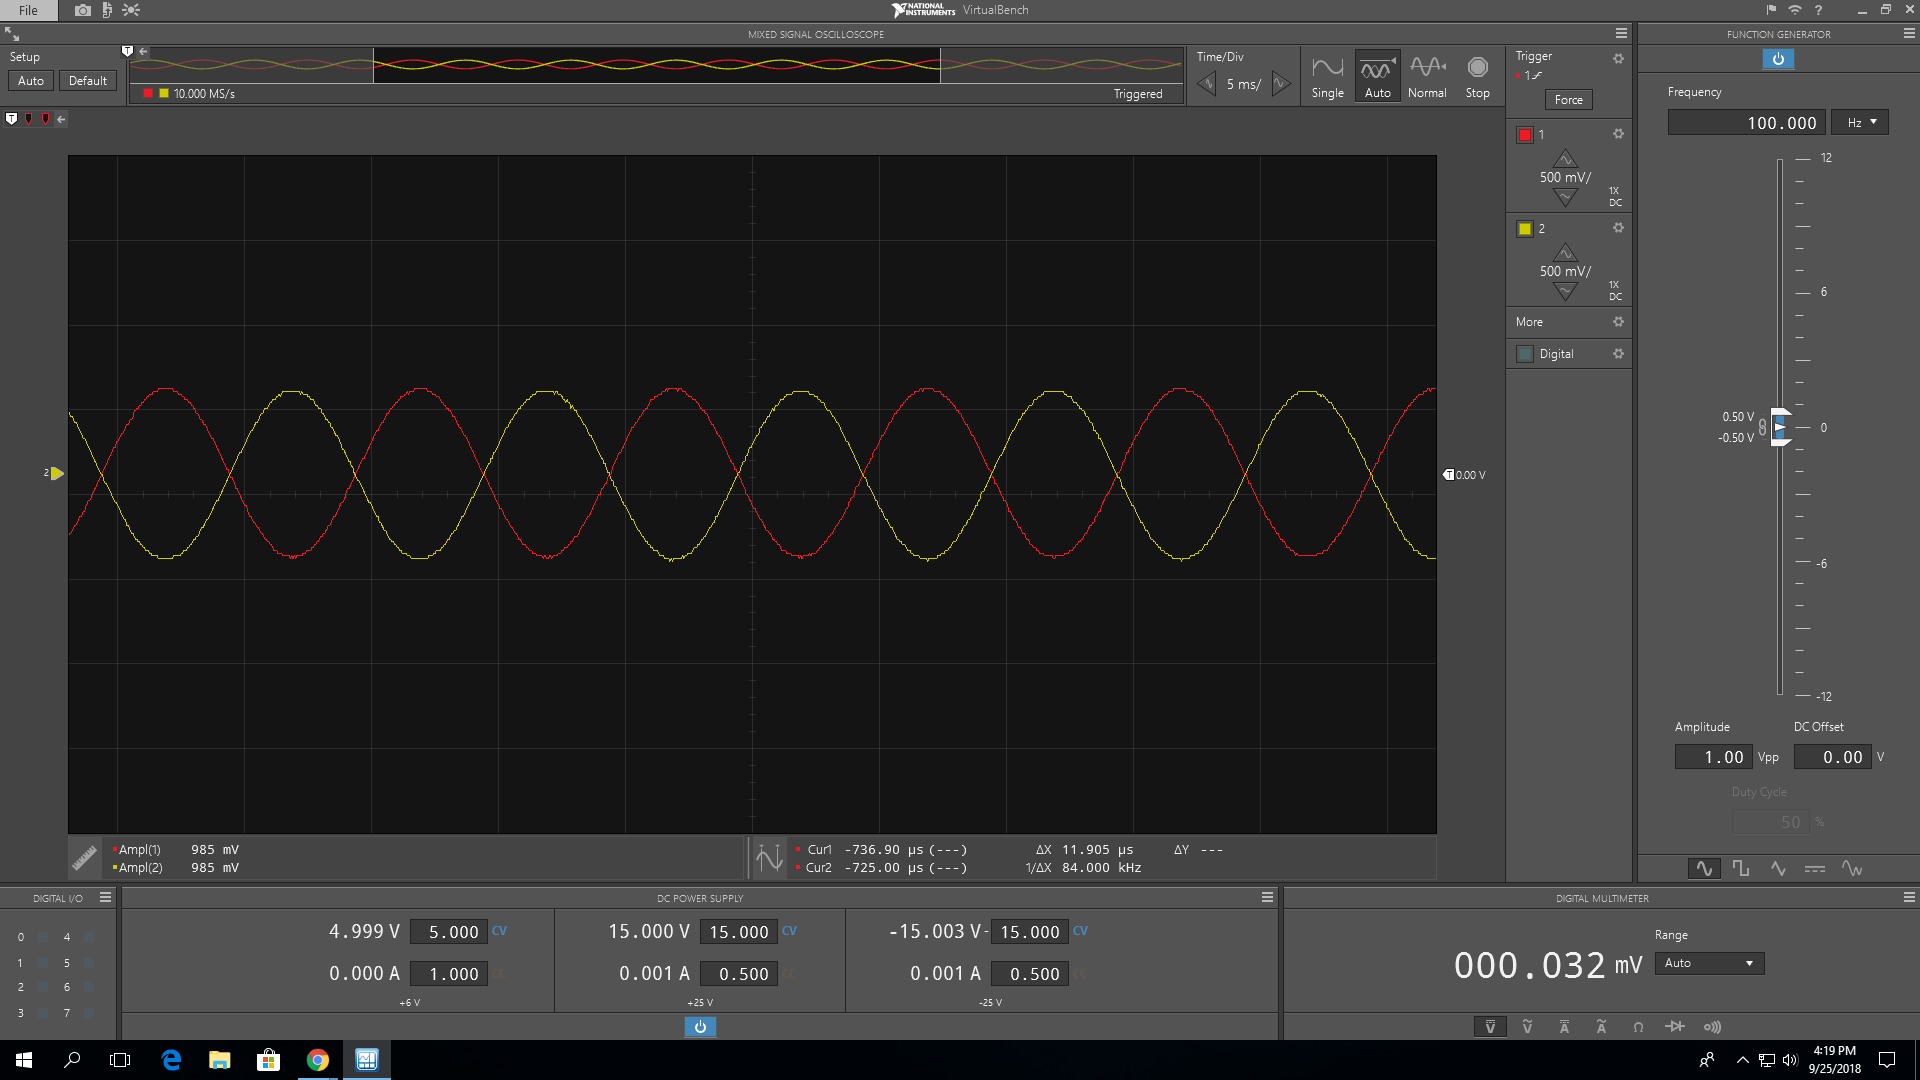
\includegraphics[scale=0.22]{images/invertingamplifier.png}
		\caption{OpAmp Output in Response to 1 $V_{pp}$, 100 Hz sine wave}				
		\label{fig:invertingamp}
	\end{figure}
\end{centering}

We then replaced the 10 $k\Omega$ resistor with a 100 $k\Omega$ resistor. The gain then became approximately 10 because $\frac{R_F}{R_1}1 = \frac{100k\Omega}{10k\Omega} = 10$. We then started to increase the amplitude of the input and noticed that clipping began to occur when $|V_{IN}| = 3$. This is the same amplitude as Experiment 1.1 because we didn't change the power supply to the Op-Amp; thus, the op-amp is limited to a 30 V range (+=15 V).

We then reduced the input amplitude so that $|V_{OUT}| = 20V$. We then began to increase the input frequency. We noticed that the peak-to-peak voltage of $v_{OUT}$ decreased to 10 V at 33 kHz. 

\quad We then set the function generator to produce a triangle and a square wave. We observed that the output to the triangle wave was also a triangle wave with no DC offset. However, when we inputted a square wave, we observed a 4V DC offset on the output (the waveform was square as well). 

\quad We then set the function generator to a 100 Hz sine wave and reduced the amplitude to produce a 1$V_{pp}$ output. We then began to increase the input frequency until $V_{pp}$ output was 0.7. This occured when the input frequency was 91 kHz, which is the true cutoff frequency of the amplifier. \\\\

\quad In Part A of Experiment 4.3, we constructed a photodiode amplifier, one type of a transresistance amplifier according to Fig. \ref{fig:transresistance}

\begin{centering}
	\begin{figure} [H]
		\centering
		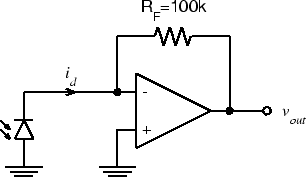
\includegraphics[scale=0.75]{images/transresistanceamplifier.png}
		\caption{Transresistance Amplifier Circuit Diagram}
		\label{fig:transresistance}
	\end{figure}
\end{centering}

When we shone a flashlight on the photodiode, we observed that $v_{OUT} = -630mV$ while without a flashlight, $v_{OUT} = -82.1 mV$. We then passed a 8 $V_{pp}$, 100 Hz sine wave into a red LED and held the red LED above the photodiode. The signal was much less distorted, appearing as below in CH2 in Fig. \ref{fig:photodiode}

\begin{centering}
	\begin{figure} [H]
		\centering
		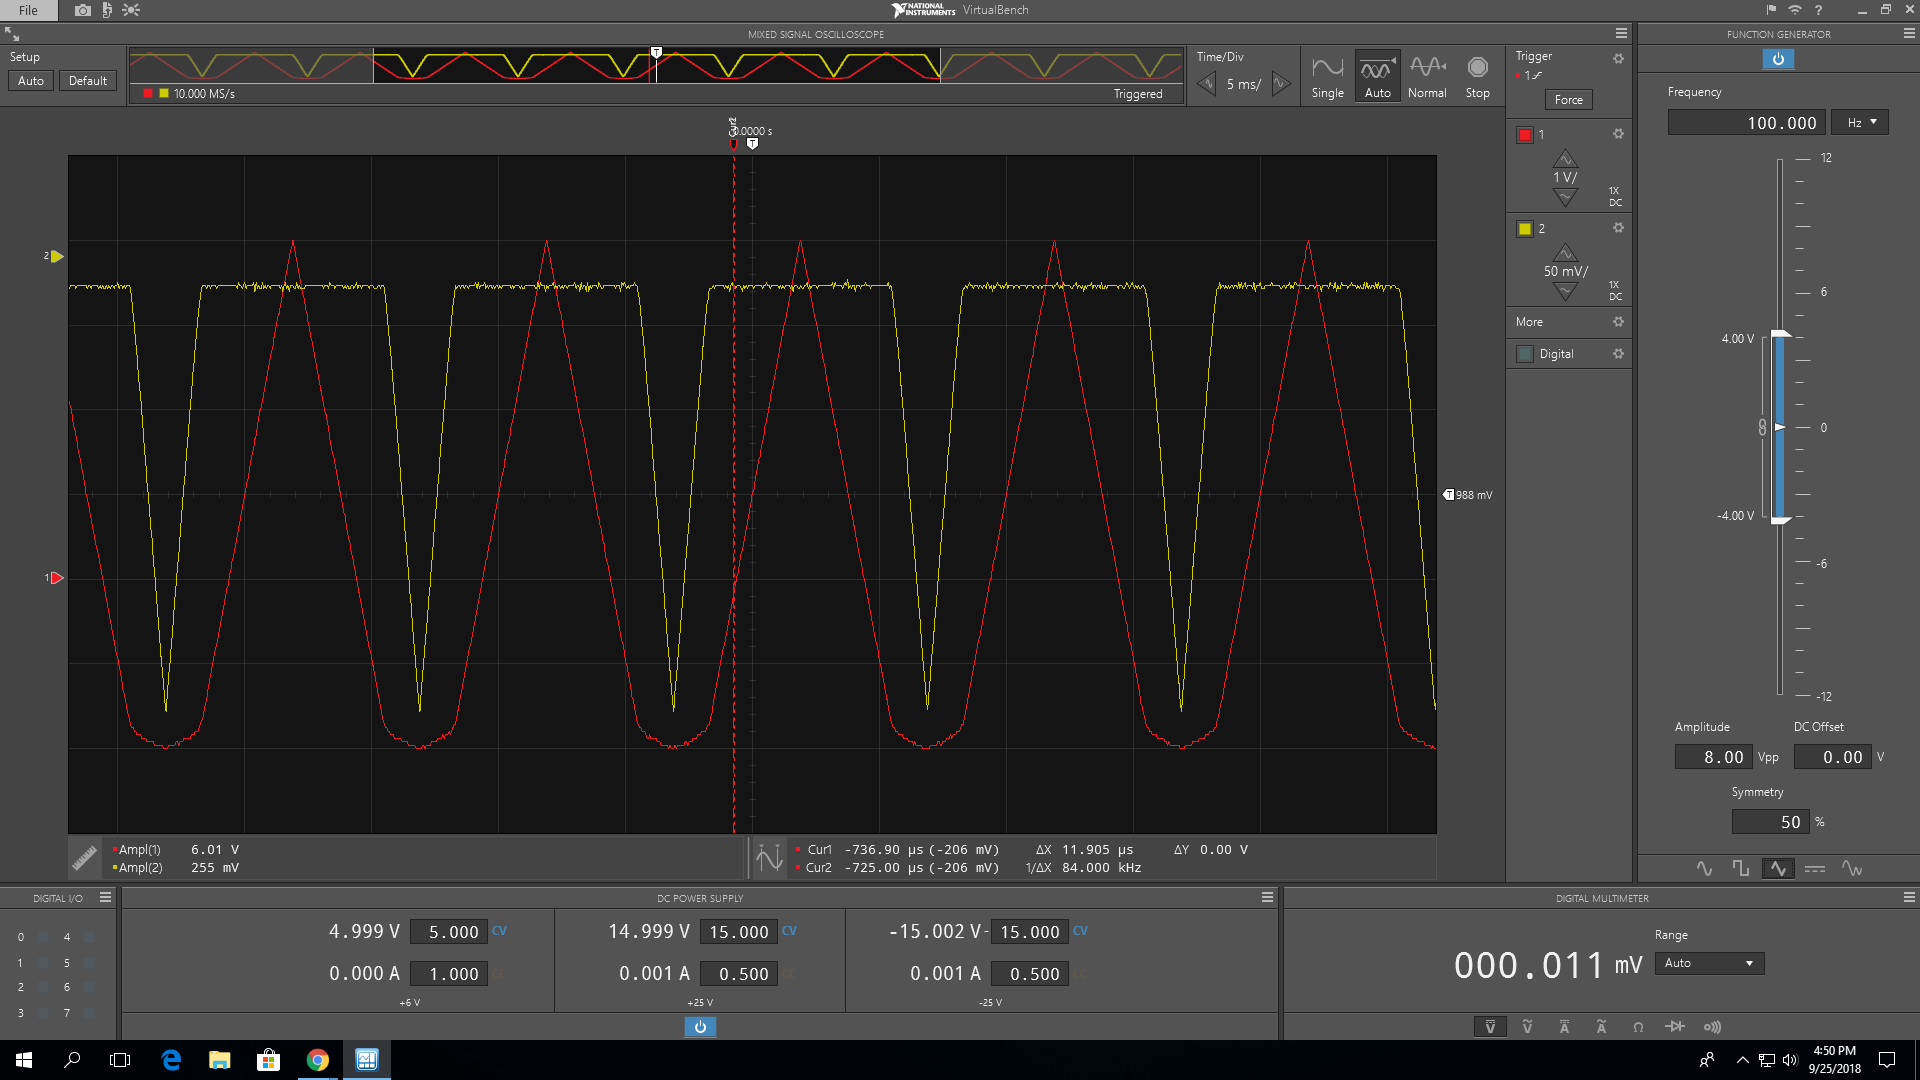
\includegraphics[scale=0.20]{images/photodiode.png}\
		\caption{Photodiode response to Red LED}
		\label{fig:photodiode}
	\end{figure}
\end{centering}

We then set the function generator to a produce a square wave of maximum amplitude, then we began moving the Red LED away from the photodiode to measure the maximum distance that the signal could still be transmitted. This distance was about 12 inches, which was a smiilar distance to that measured in Lab 2. 

We then analyzed the transresistance amplifier to show that $v_{OUT} = R_Fi_d$
We first use the current junction rule that the sum of currents coming into a node must equal zero for the central node. We then obtain the following equation: \\ 
$$i_d - \frac{V_{OUT}}{R_F} = 0$$
Solving for $v_{OUT}$ yields:
 $$V_{OUT} = i_dR_f$$
 
In part B, we amplified the gain of the microphone to a 1 $V_{pp}$ signal. In lab 2, we measured $V_{OUT}$ of the microphone to be 33 mV, which would mean that we would need a gain of $1/0.033 = 30.3$. This would mean that we need an input resistance $R_1 = R_f/G = 100k/30.3 = 3.3 k\Omega$ to amplify $V_{OUT}$ to 1 $V_{pp}$. 

In part C, we were asked to show that $v_{OUT} = -(\frac{R_F}{R_1}v_1 + \frac{R_F}{R_2}v_2)$ for the following Fig \ref{fig:mixer}

\begin{centering}
	\begin{figure} [H]
		\centering
		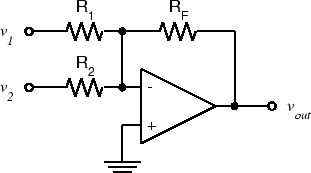
\includegraphics[scale=0.50]{images/mixercircuit.png}\
		\caption{Mixer Circuit}
		\label{fig:mixer}
	\end{figure}
\end{centering}

We begin by observing that the central node must have a voltage of zero because the positive terminal of the op-amp is connected to ground. Thus, we can use Kirchoff's current junction rule that all currents entering a junction sum to zero as follows:

$$\frac{v_2}{R_2} + \frac{v_1}{R_1} + \frac{v_{OUT}}{R_F} = 0$$

Solving for $v_{OUT}$ yields:$$v_{OUT} = -(\frac{R_F}{R_1}v_1 + \frac{R_F}{R_2}v_2)$$

We then wired the carbon microphone into the following circuit (fig \ref{fig:carbon}) where $R_{carbon}$ was the carbon microphone. 

\begin{centering}
	\begin{figure} [H]
		\centering
		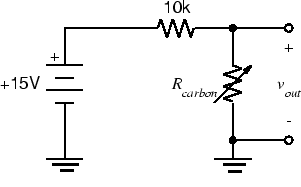
\includegraphics[scale=0.50]{images/carbonmicrophone.png}\
		\caption{Carbon Microphone Circuit}
		\label{fig:carbon}
	\end{figure}
\end{centering}

When we played an A note (440 Hz tune from a cellphone speaker), we observed that $V_{pp} = 145mV$.  

In the final portion of the lab, we combined the two circuits from the previous section to create a mixer that allowed us to hear inputs from both the carbon microphone and the dynamic microphone through the carbon phone speaker. In order to give $v_{out}$ a $V_{pp}$ of 1 V, we calculated that $R_2$ had to be 3.3 $k\Omega$

\section{References}

https://www.ece.rice.edu/~dpr2/elec240/lab4/

\section{Conclusion}

\subsection{4.1: The 741 Op Amp}
The first part of this lab was simply connecting the Op Amp to the breadboard and understanding the pins on the Op Amp. Knowing where to wire the the positive and negative power of the Op Amp is of high value since it is pretty easy to short the Op Amp and blow it out. First we just looked at various types of common waveforms and their outputs through the oscilloscope. Then we compared the open and closed loop configurations of the the Op Amp circuit and noted the difference. after the tests it was determined that closed loop was optimal since it minimized the distortions present in the Op Amp, such as not magnifying the intrinsic DC offset of the Op Amp.

\subsection{4.2: The Inverting Configuration}
The inverting amplifier worked as advertised, and when the load resistance was equal to the incident resistance, the signal was inverted with a gain of 1. When the feedback resistance was changed to ten times larger than that of $R_1$, we expected and received a gain of 10. We also found that the clipping level in this portion was, unsurprisingly, the same as that in Experiment 4.1 because of the finite voltage limitations of the 15 V power supply. When we changed the voltage input to a square and triangle wave, we found that the output waveforms were, respectively, square and triangular (but also inverted) because the omp amp merely inverted the waveform and amplified it without phase shifting. 

\subsection{4.3: Transducer Amplifiers}
When we configured the photodiode with an op-amp in this section, we found that the resulting $v_{OUT}$ square wave from the photodiode was much less distorted than that in Lab 2. We conclude that this occured because the op-amp was able to magnify the square wave from the photodiode so that it was more easily viewable and clean compared to an unamplified signal in Lab 2. Unsurprisingly, we found that the maximum distance that the LED square wave signal could be transmitted was similar to that measured in Lab 2 because we used the same photodiode, which would lead to similar transmission differences. 

\section{Errors}
\begin{itemize}
	\item \textit{Calculated value of $R_1$ does not exactly lead to gain of 1} In Experiment 4.3 Part B, we calculated a resistance value that led to a gain of slightly more than 1. This was because we played a A tone from a different file in Lab 2 than in Lab 4 which may have been softer than that for this lab. Thus, we may have selected an initial resistance value that was too low. To remedy this, we should play the note from the same audio file at the same volume for higher consistency. 
	\item \textit{Large DC Offset on the open-loop response circuit} We found that the DC offset on the open-loop response circuit to be over 70 mV, which was extremely high. Though much of this was due to the nature of the circuit itself, we concluded that the op-amp itself created a significant amount of DC offset. We believe that using a newer op-amp with a smaller DC offset would result in a smaller DC offset for $V_{out}$. 
\end{itemize}


\medskip

%\textit{Note (To be deleted): Briefly list sources of error and discuss how to eliminate or deal with them}

\end{document}
